\documentclass{article}
\usepackage[paperwidth=20cm,paperheight=18cm,margin=0.5cm]{geometry}
\usepackage{tikz}
\usepackage{xcolor}
\begin{document}
\pagestyle{empty}
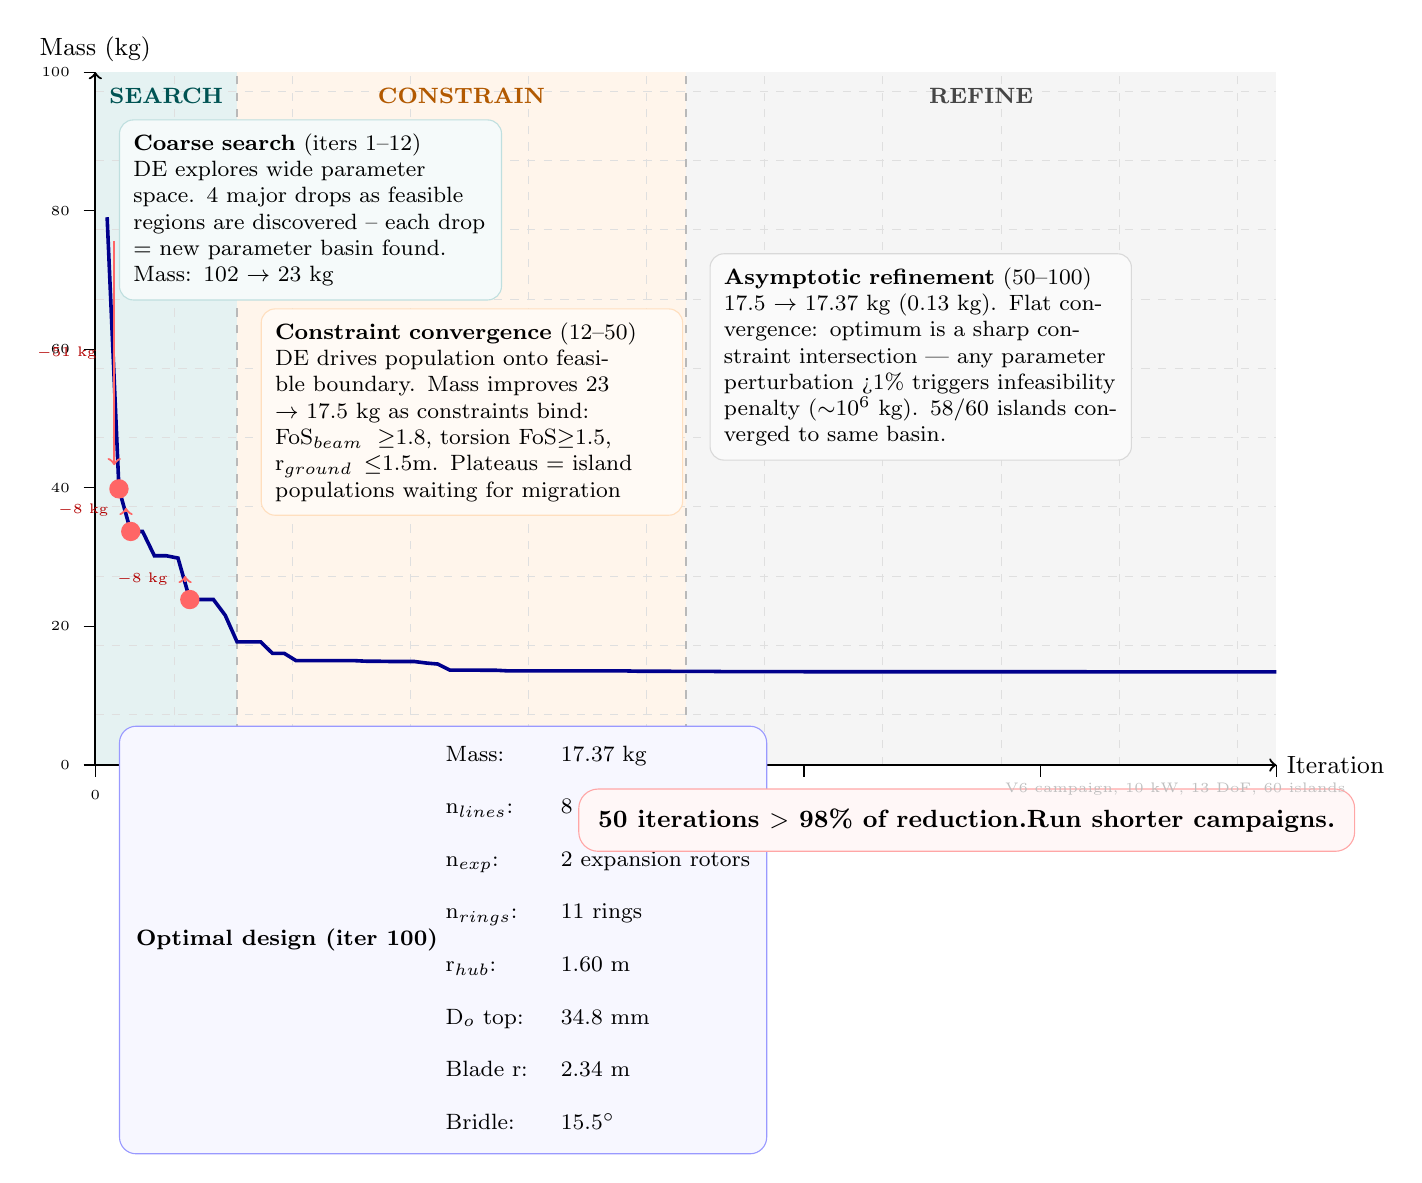
\begin{tikzpicture}[scale=1.0]

% Phase regions
\fill[teal!10] (2.0,2.0) rectangle (3.8,10.8);
\fill[orange!8] (3.8,2.0) rectangle (9.5,10.8);
\fill[gray!8] (9.5,2.0) rectangle (17.0,10.8);

\draw[gray!25, very thin, dashed] (2.0,2.0) grid[xstep=1.5,ystep=0.88] (17.0,10.8);

\draw[thick, ->] (2.0,2.0) -- (17.0,2.0) node[right, font=\small] {Iteration};
\draw[thick, ->] (2.0,2.0) -- (2.0,10.8) node[above, font=\small] {Mass (kg)};
\foreach \y/\l in {2.0/0, 3.76/20, 5.52/40, 7.28/60, 9.04/80, 10.8/100} {\draw (1.85,\y) -- (2.0,\y); \node[left, font=\tiny] at (1.8,\y) {\l};}
\foreach \x/\l in {2.0/0, 5.0/20, 8.0/40, 11.0/60, 14.0/80, 17.0/100} {\draw (\x,1.85) -- (\x,2.0); \node[below, font=\tiny] at (\x,1.8) {\l};}

\draw[dashed, thick, gray!55] (3.8,2.0) -- (3.8,10.8);
\draw[dashed, thick, gray!55] (9.5,2.0) -- (9.5,10.8);
\node[font=\footnotesize\bfseries, teal!65!black] at (2.9,10.5) {SEARCH};
\node[font=\footnotesize\bfseries, orange!70!black] at (6.65,10.5) {CONSTRAIN};
\node[font=\footnotesize\bfseries, gray!55!black] at (13.25,10.5) {REFINE};

\draw[blue!55!black, line width=1.3pt] plot coordinates {
    (2.1500,8.9572)%
    (2.3000,5.5076)%
    (2.4500,4.9665)%
    (2.6000,4.9665)%
    (2.7500,4.6581)%
    (2.9000,4.6581)%
    (3.0500,4.6284)%
    (3.2000,4.1019)%
    (3.3500,4.1019)%
    (3.5000,4.1019)%
    (3.6500,3.9013)%
    (3.8000,3.5642)%
    (3.9500,3.5642)%
    (4.1000,3.5640)%
    (4.2500,3.4179)%
    (4.4000,3.4179)%
    (4.5500,3.3255)%
    (4.7000,3.3255)%
    (4.8500,3.3255)%
    (5.0000,3.3255)%
    (5.1500,3.3255)%
    (5.3000,3.3255)%
    (5.4500,3.3181)%
    (5.6000,3.3181)%
    (5.7500,3.3151)%
    (5.9000,3.3151)%
    (6.0500,3.3151)%
    (6.2000,3.2959)%
    (6.3500,3.2826)%
    (6.5000,3.2062)%
    (6.6500,3.2062)%
    (6.8000,3.2062)%
    (6.9500,3.2033)%
    (7.1000,3.2033)%
    (7.2500,3.1954)%
    (7.4000,3.1954)%
    (7.5500,3.1954)%
    (7.7000,3.1954)%
    (7.8500,3.1954)%
    (8.0000,3.1954)%
    (8.1500,3.1954)%
    (8.3000,3.1954)%
    (8.4500,3.1954)%
    (8.6000,3.1952)%
    (8.7500,3.1952)%
    (8.9000,3.1911)%
    (9.0500,3.1911)%
    (9.2000,3.1911)%
    (9.3500,3.1904)%
    (9.5000,3.1904)%
    (9.6500,3.1904)%
    (9.8000,3.1895)%
    (9.9500,3.1873)%
    (10.1000,3.1873)%
    (10.2500,3.1873)%
    (10.4000,3.1873)%
    (10.5500,3.1873)%
    (10.7000,3.1873)%
    (10.8500,3.1873)%
    (11.0000,3.1854)%
    (11.1500,3.1854)%
    (11.3000,3.1854)%
    (11.4500,3.1854)%
    (11.6000,3.1854)%
    (11.7500,3.1854)%
    (11.9000,3.1854)%
    (12.0500,3.1854)%
    (12.2000,3.1854)%
    (12.3500,3.1854)%
    (12.5000,3.1853)%
    (12.6500,3.1853)%
    (12.8000,3.1852)%
    (12.9500,3.1852)%
    (13.1000,3.1852)%
    (13.2500,3.1852)%
    (13.4000,3.1851)%
    (13.5500,3.1848)%
    (13.7000,3.1846)%
    (13.8500,3.1844)%
    (14.0000,3.1844)%
    (14.1500,3.1844)%
    (14.3000,3.1844)%
    (14.4500,3.1844)%
    (14.6000,3.1842)%
    (14.7500,3.1842)%
    (14.9000,3.1842)%
    (15.0500,3.1842)%
    (15.2000,3.1842)%
    (15.3500,3.1842)%
    (15.5000,3.1842)%
    (15.6500,3.1842)%
    (15.8000,3.1842)%
    (15.9500,3.1842)%
    (16.1000,3.1842)%
    (16.2500,3.1842)%
    (16.4000,3.1842)%
    (16.5500,3.1842)%
    (16.7000,3.1842)%
    (16.8500,3.1842)%
    (17.0000,3.1842)
};

  \fill[red!60] (2.3000,5.5076) circle (3.5pt);
  \fill[red!60] (2.4500,4.9665) circle (3.5pt);
  \fill[red!60] (3.2000,4.1019) circle (3.5pt);

  \draw[->, red!60, line width=0.8pt] (2.2400,8.6572) -- (2.2400,5.8076);
  \node[font=\tiny, red!70!black, anchor=east] at (2.1400,7.2324) {$-$51 kg};
  \draw[->, red!60, line width=0.8pt] (2.3900,5.2076) -- (2.3900,5.2665);
  \node[font=\tiny, red!70!black, anchor=east] at (2.2900,5.2370) {$-$8 kg};
  \draw[->, red!60, line width=0.8pt] (3.1400,4.3284) -- (3.1400,4.4019);
  \node[font=\tiny, red!70!black, anchor=east] at (3.0400,4.3651) {$-$8 kg};


% Coarse search box
\node[font=\footnotesize, anchor=north west, fill=teal!4, draw=teal!25, rounded corners=5pt, inner sep=5pt, text width=4.5cm] at (2.3, 10.2) {\textbf{Coarse search} (iters 1--12)\\ DE explores wide parameter space. 4 major drops as feasible regions are discovered -- each drop = new parameter basin found. Mass: 102 $\rightarrow$ 23 kg};

% Constraint box
\node[font=\footnotesize, anchor=north west, fill=orange!4, draw=orange!25, rounded corners=5pt, inner sep=5pt, text width=5.0cm] at (4.1, 7.8) {\textbf{Constraint convergence} (12--50)\\ DE drives population onto feasible boundary. Mass improves 23 $\rightarrow$ 17.5 kg as constraints bind: FoS$_{\text{beam}}\ge$1.8, torsion FoS$\ge$1.5, r$_{\text{ground}}\le$1.5m. Plateaus = island populations waiting for migration};

% Refinement box
\node[font=\footnotesize, anchor=north west, fill=gray!4, draw=gray!30, rounded corners=5pt, inner sep=5pt, text width=5.0cm] at (9.8, 8.5) {\textbf{Asymptotic refinement} (50--100)\\ 17.5 $\rightarrow$ 17.37 kg (0.13 kg). Flat convergence: optimum is a sharp constraint intersection --- any parameter perturbation >1\% triggers infeasibility penalty ($\sim$10$^6$ kg). 58/60 islands converged to same basin.};

% Best design
\node[font=\footnotesize, anchor=north west, fill=blue!3, draw=blue!40, rounded corners=6pt, inner sep=6pt] at (2.3, 2.5) {
  \textbf{Optimal design (iter 100)} \\[2pt]
  \begin{tabular}{@{}ll@{}}
  Mass:     & 17.37 kg \\ \\
      n$_\text{lines}$: & 8 (octagon) \\ \\
      n$_\text{exp}$:   & 2 expansion rotors \\ \\
      n$_\text{rings}$: & 11 rings \\ \\
      r$_\text{hub}$:   & 1.60 m \\ \\
      D$_o$ top:& 34.8 mm \\ \\
      Blade r:  & 2.34 m \\ \\
      Bridle:   & 15.5$^\circ$ \\
  \end{tabular}};

\node[font=\small\bfseries, anchor=east, fill=red!3, draw=red!35, rounded corners=7pt, inner sep=7pt] at (18.0, 1.3) {50 iterations $>$ 98\% of reduction.\\ Run shorter campaigns.};
\node[font=\tiny, anchor=north east, text=gray!50] at (18.0, 1.9) {V6 campaign, 10 kW, 13 DoF, 60 islands};

\end{tikzpicture}
\end{document}
